% questions.tex —— 2014 年全国Ⅱ卷（理科） · 题目内容片段（无答案）
% 由 tools/generate_projects.py 依来源总账自 2014/2014_数学真题_全国2理_试题.md 生成，勿手改（改源 MD 后重跑）


\gkpart{数学}

\begin{gktip}
\textbf{来源说明}：本题面依据固定源 PDF 两页 A3 题面逐题转录，原卷印刷页码 903–904。固定源只含试题和作答空白，不附答案或解析；答案和解析均由本库独立复算。

\textbf{图形说明}：第 6、7、18、19、22 题的题面图形在 LaTeX 工程中以 TikZ 矢量源重绘。题面中的图片标记仅为转换器定位这些矢量源的标记，仓库不保存 PNG、JPEG 或 SVG 图形文件。
\end{gktip}

\gkpart{一、选择题}

\begin{question}
\gkti{1}设集合 $M=\{0,1,2\}$，$N=\{x\mid x^2-3x+2\leqslant0\}$，则 $M\cap N=$\mbox{（　　）}

（A）$\{1\}$　　（B）$\{2\}$　　（C）$\{0,1\}$　　（D）$\{1,2\}$

\end{question}
\begin{question}
\gkti{2}设复数 $z_1,z_2$ 在复平面内的对应点关于虚轴对称，$z_1=2+i$，则 $z_1z_2=$\mbox{（　　）}

（A）$-5$　　（B）$5$　　（C）$-4+i$　　（D）$-4-i$

\end{question}
\begin{question}
\gkti{3}设向量 $\boldsymbol a,\boldsymbol b$ 满足 $|\boldsymbol a+\boldsymbol b|=\sqrt{10}$，$|\boldsymbol a-\boldsymbol b|=\sqrt6$，则 $\boldsymbol a\cdot\boldsymbol b=$\mbox{（　　）}

（A）$1$　　（B）$2$　　（C）$3$　　（D）$5$

\end{question}
\begin{question}
\gkti{4}钝角三角形 $ABC$ 的面积是 $\dfrac12$，$AB=1$，$BC=\sqrt2$，则 $AC=$\mbox{（　　）}

（A）$5$　　（B）$\sqrt5$　　（C）$2$　　（D）$1$

\end{question}
\begin{question}
\gkti{5}某地区空气质量监测资料表明，一天的空气质量为优良的概率是 $0.75$，连续两天为优良的概率是 $0.6$，已知某天的空气质量为优良，则随后一天的空气质量为优良的概率是\mbox{（　　）}

（A）$0.8$　　（B）$0.75$　　（C）$0.6$　　（D）$0.45$

\Needspace{0.4\textheight}
\end{question}
\begin{question}
\gkti{6}如图，网格纸上正方形小格的边长为 $1$（表示 $1\ \mathrm{cm}$），图中粗线画出的是某零件的三视图，该零件由一个底面半径为 $3\ \mathrm{cm}$，高为 $6\ \mathrm{cm}$ 的圆柱体毛坯切削得到，则切削掉的部分的体积与原来毛坯体积的比值为\mbox{（　　）}
\nopagebreak[4]
\begin{center}% 2014 全国卷Ⅱ理科第 6 题：圆柱零件的三视图（方格边长表示 1 cm）。
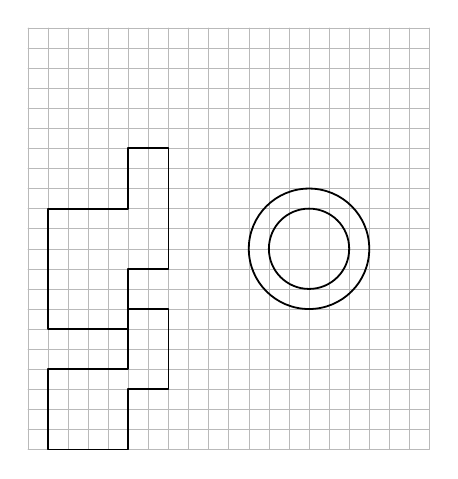
\begin{tikzpicture}[x=2.55mm,y=2.55mm,line cap=round,line join=round]
  % 细灰色方格与题给粗实线分层；原图没有虚线。
  \draw[step=1,gray!55,line width=.18pt] (0,-3) grid (20,18);
  % 左上、左下阶梯投影。
  \draw[line width=.65pt] (1,9)--(5,9)--(5,12)--(7,12)--(7,6)--(5,6)--(5,3)--(1,3)--cycle;
  \draw[line width=.65pt] (1,1)--(5,1)--(5,4)--(7,4)--(7,0)--(5,0)--(5,-3)--(1,-3)--cycle;
  % 右上投影：两个同心圆，圆心在同一方格交点。
  \draw[line width=.65pt] (14,7) circle[radius=3];
  \draw[line width=.65pt] (14,7) circle[radius=2];
\end{tikzpicture}
\end{center}
\nopagebreak[4]
（A）$\dfrac{17}{27}$　　（B）$\dfrac59$　　（C）$\dfrac{10}{27}$　　（D）$\dfrac13$

\Needspace{0.4\textheight}
\end{question}
\begin{question}
\gkti{7}执行如图所示的程序框图，如果输入的 $x,t$ 均为 $2$，则输出的 $S=$\mbox{（　　）}
\nopagebreak[4]
\begin{center}% 2014 全国卷Ⅱ理科第 7 题：累加计算程序框图。
\begin{tikzpicture}[font=\footnotesize,>=Stealth,node distance=4mm,line width=.4pt,
  box/.style={draw,minimum height=1.65em,minimum width=7.0em,inner xsep=4pt},
  term/.style={draw,rounded corners=6pt,minimum height=1.65em,inner xsep=8pt},
  io/.style={draw,trapezium,trapezium left angle=70,trapezium right angle=110,
             minimum height=1.65em,inner xsep=4pt},
  dec/.style={draw,diamond,aspect=2.25,inner sep=1.6pt}]
  \node[term] (start) {开始};
  \node[io,below=of start] (input) {输入 $x,t$};
  \node[box,below=of input] (init) {$M=1,\ S=3$};
  \node[box,below=of init] (kinit) {$k=1$};
  \node[dec,below=7mm of kinit] (cond) {$k\leqslant t$};
  \node[box,below left=9mm and 16mm of cond] (calc) {$M=\dfrac{M}{k}x$};
  \node[box,below=of calc] (sum) {$S=M+S$};
  \node[box,below=of sum] (inc) {$k=k+1$};
  \node[io,below right=9mm and 16mm of cond] (output) {输出 $S$};
  \node[term,below=of output] (end) {结束};
  \draw[->] (start)--(input)--(init)--(kinit)--(cond);
  \draw[->] (cond.south west)--node[left] {是}(calc)--(sum)--(inc);
  \draw[->] (inc.west)-| ([xshift=-48mm]cond.west) |- (cond.north);
  \draw[->] (cond.south east)--node[right] {否}(output)--(end);
\end{tikzpicture}
\end{center}
\nopagebreak[4]
（A）$4$　　（B）$5$　　（C）$6$　　（D）$7$

\end{question}
\begin{question}
\gkti{8}设曲线 $y=ax-\ln(x+1)$ 在点 $(0,0)$ 处的切线方程为 $y=2x$，则 $a=$\mbox{（　　）}

（A）$0$　　（B）$1$　　（C）$2$　　（D）$3$

\end{question}
\begin{question}
\gkti{9}设 $x,y$ 满足约束条件

\nopagebreak[4]
\[
\begin{cases}
x+y-7\leqslant0,\\
x-3y+1\leqslant0,\\
3x-y-5\geqslant0,
\end{cases}
\]

则 $z=2x-y$ 的最大值为\mbox{（　　）}

（A）$10$　　（B）$8$　　（C）$3$　　（D）$2$

\end{question}
\begin{question}
\gkti{10}设 $F$ 为抛物线 $C:y^2=3x$ 的焦点，过 $F$ 且倾斜角为 $30^\circ$ 的直线交 $C$ 于 $A,B$ 两点，$O$ 为坐标原点，则 $\triangle OAB$ 的面积为\mbox{（　　）}

（A）$\dfrac{3\sqrt3}{4}$　　（B）$\dfrac{9\sqrt3}{8}$　　（C）$\dfrac{63}{32}$　　（D）$\dfrac94$

\end{question}
\begin{question}
\gkti{11}直三棱柱 $ABC-A_1B_1C_1$ 中，$\angle BCA=90^\circ$，$M,N$ 分别是 $A_1B_1,A_1C_1$ 的中点，$BC=CA=CC_1$，则 $BM$ 与 $AN$ 所成角的余弦值为\mbox{（　　）}

（A）$\dfrac1{10}$　　（B）$\dfrac25$　　（C）$\dfrac{\sqrt{30}}{10}$　　（D）$\dfrac{\sqrt2}{2}$

\end{question}
\begin{question}
\gkti{12}设函数 $f(x)=\sqrt3\sin\dfrac{\pi x}{m}$，若存在 $f(x)$ 的极值点 $x_0$ 满足 $x_0^2+[f(x_0)]^2<m^2$，则 $m$ 的取值范围是\mbox{（　　）}

（A）$(-\infty,-6)\cup(6,+\infty)$　　（B）$(-\infty,-4)\cup(4,+\infty)$

（C）$(-\infty,-2)\cup(2,+\infty)$　　（D）$(-\infty,-1)\cup(1,+\infty)$

\end{question}
\gkpart{二、填空题}

\begin{question}
\gkti{13}$(x+a)^{10}$ 的展开式中，$x^7$ 的系数为 $15$，则 $a=$\gkblank{}。（用数字填写答案）

\end{question}
\begin{question}
\gkti{14}函数 $f(x)=\sin(x+2\varphi)-2\sin\varphi\cos(x+\varphi)$ 的最大值为\gkblank{}。

\end{question}
\begin{question}
\gkti{15}已知偶函数 $f(x)$ 在 $[0,+\infty)$ 单调递减，$f(2)=0$，若 $f(x-1)>0$，则 $x$ 的取值范围是\gkblank{}。

\end{question}
\begin{question}
\gkti{16}设点 $M(x_0,1)$，若在圆 $O:x^2+y^2=1$ 上存在点 $N$，使得 $\angle OMN=45^\circ$，则 $x_0$ 的取值范围是\gkblank{}。

\end{question}
\gkpart{三、解答题}

\begin{question}
\gkti{17}已知数列 $\{a_n\}$ 满足 $a_1=1$，$a_{n+1}=3a_n+1$。

(1) 证明 $\left\{a_n+\dfrac12\right\}$ 是等比数列，并求 $\{a_n\}$ 的通项公式；

(2) 证明：$\dfrac1{a_1}+\dfrac1{a_2}+\cdots+\dfrac1{a_n}<\dfrac32$。

\Needspace{0.4\textheight}
\end{question}
\begin{question}
\gkti{18}如图，四棱锥 $P-ABCD$ 中，底面 $ABCD$ 为矩形，$PA\perp$ 平面 $ABCD$，$E$ 为 $PD$ 的中点。
\nopagebreak[4]
\begin{center}% 2014 全国卷Ⅱ理科第 18 题：四棱锥 P-ABCD，E 为 PD 中点。
\begin{tikzpicture}[font=\footnotesize,line width=.45pt,line cap=round,line join=round]
  \coordinate (A) at (0,0);
  \coordinate (B) at (-1.20,-1.70);
  \coordinate (C) at (3.35,-1.70);
  \coordinate (D) at (4.55,0);
  \coordinate (P) at (0,4.25);
  \coordinate (E) at ($(P)!0.5!(D)$);
  % 题面可见棱及辅助线。
  \draw (P)--(B)--(C)--(D)--(P);
  \draw (P)--(C) (P)--(E) (E)--(C);
  % 经过 A 的底面后边、PA 及其辅助连线为不可见线。
  \draw[dashed] (P)--(A)--(B) (A)--(D) (A)--(C) (A)--(E);
  \node[left] at (P) {$P$};
  \node[above left] at (A) {$A$};
  \node[below left] at (B) {$B$};
  \node[below right] at (C) {$C$};
  \node[right] at (D) {$D$};
  \node[right] at (E) {$E$};
\end{tikzpicture}
\end{center}
\nopagebreak[4]
(1) 证明：$PB\parallel$ 平面 $AEC$；

(2) 设二面角 $D-AE-C$ 为 $60^\circ$，$AP=1$，$AD=\sqrt3$，求三棱锥 $E-ACD$ 的体积。

\par\medskip

*以下续自固定源 PDF 第 2 页（印刷页 904）。*

\Needspace{0.4\textheight}
\end{question}
\begin{question}
\gkti{19}某地区 $2007$ 年至 $2013$ 年农村居民家庭人均纯收入 $y$（单位：千元）的数据如下表：
\nopagebreak[4]
\begin{center}% 2014 全国卷Ⅱ理科第 19 题：2007--2013 年农村居民家庭人均纯收入数据表。
% 单位为千元；三行八列的 entries 与题面逐项对应。
\begin{tikzpicture}[font=\footnotesize,baseline=(current bounding box.center)]
  % 首列较宽，其余七列等宽；只用普通路径和文字节点绘制表格。
  \draw (0,0) rectangle (9.40,2.70);
  \draw (2.75,0)--(2.75,2.70);
  \draw (3.70,0)--(3.70,2.70);
  \draw (4.65,0)--(4.65,2.70);
  \draw (5.60,0)--(5.60,2.70);
  \draw (6.55,0)--(6.55,2.70);
  \draw (7.50,0)--(7.50,2.70);
  \draw (8.45,0)--(8.45,2.70);
  \draw (0,0.90)--(9.40,0.90);
  \draw (0,1.80)--(9.40,1.80);

  \node at (1.375,2.25) {年份};
  \node at (3.225,2.25) {2007};
  \node at (4.175,2.25) {2008};
  \node at (5.125,2.25) {2009};
  \node at (6.075,2.25) {2010};
  \node at (7.025,2.25) {2011};
  \node at (7.975,2.25) {2012};
  \node at (8.925,2.25) {2013};

  \node at (1.375,1.35) {年份代号 $t$};
  \node at (3.225,1.35) {1};
  \node at (4.175,1.35) {2};
  \node at (5.125,1.35) {3};
  \node at (6.075,1.35) {4};
  \node at (7.025,1.35) {5};
  \node at (7.975,1.35) {6};
  \node at (8.925,1.35) {7};

  \node at (1.375,0.45) {人均纯收入 $y$};
  \node at (3.225,0.45) {2.9};
  \node at (4.175,0.45) {3.3};
  \node at (5.125,0.45) {3.6};
  \node at (6.075,0.45) {4.4};
  \node at (7.025,0.45) {4.8};
  \node at (7.975,0.45) {5.2};
  \node at (8.925,0.45) {5.9};
  \node[anchor=south east] at (9.40,2.95) {单位：千元};
\end{tikzpicture}
\end{center}
\nopagebreak[4]
为避免转换时丢失题面数据，表中三行全部 entries、单位和行列语义逐项转录如下：

\begin{center}
\begingroup\setlength{\tabcolsep}{4pt}
\begin{tabular}{llllllll}
\toprule
年份 & 2007 & 2008 & 2009 & 2010 & 2011 & 2012 & 2013 \\
\midrule
年份代号 $t$ & 1 & 2 & 3 & 4 & 5 & 6 & 7 \\
人均纯收入 $y$（千元） & 2.9 & 3.3 & 3.6 & 4.4 & 4.8 & 5.2 & 5.9 \\
\bottomrule
\end{tabular}
\endgroup
\end{center}

(1) 求 $y$ 关于 $t$ 的线性回归方程；

(2) 利用 (1) 中的回归方程，分析 $2007$ 年至 $2013$ 年该地区农村居民家庭人均纯收入的变化情况，并预测该地区 $2015$ 年农村居民家庭人均纯收入。

\Needspace{5\baselineskip}
附：回归直线的斜率和截距的最小二乘估计公式分别为：

\nopagebreak[4]
\[
\hat b=\frac{\sum_{i=1}^n(t_i-\bar t)(y_i-\bar y)}{\sum_{i=1}^n(t_i-\bar t)^2},\qquad \hat a=\bar y-\hat b\bar t.
\]

\end{question}
\begin{question}
\gkti{20}设 $F_1,F_2$ 分别是椭圆 $C:\dfrac{x^2}{a^2}+\dfrac{y^2}{b^2}=1\ (a>b>0)$ 的左、右焦点，$M$ 是 $C$ 上一点且 $MF_2$ 与 $x$ 轴垂直，直线 $MF_1$ 与 $C$ 的另一个交点为 $N$。

(1) 若直线 $MN$ 的斜率为 $\dfrac34$，求 $C$ 的离心率；

(2) 若直线 $MN$ 在 $y$ 轴上的截距为 $2$，且 $|MN|=5|F_1N|$，求 $a,b$。

\end{question}
\begin{question}
\gkti{21}已知函数 $f(x)=e^x-e^{-x}-2x$。

(1) 讨论 $f(x)$ 的单调性；

(2) 设 $g(x)=f(2x)-4bf(x)$，当 $x>0$ 时，$g(x)>0$，求 $b$ 的最大值；

(3) 已知 $1.4142<\sqrt2<1.4143$，估计 $\ln2$ 的近似值（精确到 $0.001$）。

\Needspace{0.4\textheight}
\end{question}
\begin{question}
\gkti{22}如图，$P$ 是 $\odot O$ 外一点，$PA$ 是切线，$A$ 为切点，割线 $PBC$ 与 $\odot O$ 相交于点 $B,C$，$PC=2PA$，$D$ 为 $PC$ 的中点，$AD$ 的延长线交 $\odot O$ 于点 $E$。证明：
\nopagebreak[4]
\begin{center}% 2014 全国卷Ⅱ理科第 22 题：切线、割线及 A-D-E 辅助线。
\begin{tikzpicture}[font=\footnotesize,line width=.45pt,line cap=round,line join=round]
  \coordinate (O) at (0,0);
  \coordinate (P) at (-3.000,-1.225);
  \coordinate (B) at (-1.935,-1.420);
  \coordinate (C) at (1.307,-2.013);
  \coordinate (D) at ($(P)!0.5!(C)$);
  \coordinate (A) at (-2.255,.821);
  \coordinate (E) at (-.417,-2.364);
  \draw (O) circle[radius=2.40];
  \draw (P)--(A);
  \draw (P)--(C);
  \draw (A)--(E);
  \fill (O) circle (1.15pt);
  \node[left] at (P) {$P$};
  \node[left] at (A) {$A$};
  \node[below left] at (B) {$B$};
  \node[below right] at (C) {$C$};
  \node[above right] at (D) {$D$};
  \node[below] at (E) {$E$};
  \node[right] at (O) {$O$};
\end{tikzpicture}
\end{center}
\nopagebreak[4]
(1) $BE=EC$；

(2) $AD\cdot DE=2PB^2$。

\end{question}
\begin{question}
\gkti{23}在直角坐标系 $xOy$ 中，以坐标原点为极点，$x$ 轴正半轴为极轴建立极坐标系，半圆 $C$ 的极坐标方程为 $\rho=2\cos\theta$，$\theta\in\left[0,\dfrac\pi2\right]$。

(1) 求 $C$ 的参数方程；

(2) 设点 $D$ 在 $C$ 上，$C$ 在 $D$ 处的切线与直线 $l:y=\sqrt3x+2$ 垂直，根据 (1) 中你得到的参数方程，确定点 $D$ 的坐标。

\end{question}
\begin{question}
\gkti{24}设函数 $f(x)=\left|x+\dfrac1a\right|+|x-a|\ (a>0)$。

(1) 证明：$f(x)\geqslant2$；

(2) 若 $f(3)<5$，求 $a$ 的取值范围。

\end{question}